\section{Introduction}\label{sec:intro}


The success of deep models in semantic segmentation~\cite{fcn, unet, pspnet, deeplab} benefits from large-scale datasets.
%
However, popular datasets for segmentation, such as PASCAL VOC~\cite{voc} and Cityscapes~\cite{cityscapes}, usually follow a long-tail distribution, where some categories may have far fewer samples than others.
%
Considering the particularity of this task, which targets assigning labels to pixels instead of images, it is quite difficult to balance the distribution from the aspect of data collection.
%
Taking the scenario of autonomous driving as an example, a bike is typically tied to a smaller image region (\textit{i.e.}, fewer pixels) than a car, and trains appear more rarely than pedestrians in a city.
%
Therefore, learning a decent model from long tail data distributions becomes critical.


% Deep learning has made incredible progress in various computer vision tasks, such as image classification, object detection and semantic segmentation.
% %
% The keys to this success are the large-scale datasets, high-performance GPUs and advancement of neural network architectures.
% %
% In real-world applications, training data typically follows a long-tailed categorical distribution, where some categories are extremely numerous and others are extremely few.
% %
% This imbalance data distribution leads to challenging model training by empirical risk minimization, making the trained model biased towards head category and causing poor performance on tail category.
% %
% Semantic segmentation, as one of the most instance-intensive task, suffers badly from the undesirable consequences of long-tailed distributions.


\definecolor{myyellow}{RGB}{184,146,48}
\definecolor{myblue}{RGB}{0,0,255}
\begin{figure}[t]
    \centering
    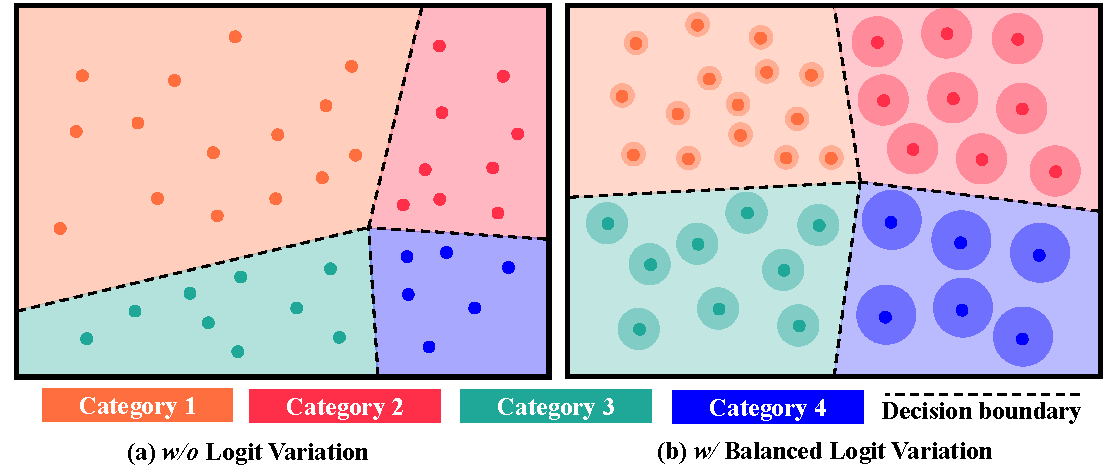
\includegraphics[width=1.0\linewidth]{figures/Motivation.pdf}
    \vspace{-15pt}
    \caption{%
        \textbf{Illustration of logit variation} from the feature space, where each point corresponds to an instance and different colors stand for different categories.
        %
        (a) Without logit variation, the features of tail classes (\textit{e.g.}, the \textbf{\textcolor{myblue}{blue}} one) may get squeezed into a narrow area.
        %
        (b) After introducing logit variation, which is controlled by the category scale (\textit{i.e.}, number of training samples belonging to a particular category), we expand each feature point to a feature region with random perturbation, resulting in a more category-balanced feature distribution.
    }
    \label{fig:stats}
    \vspace{-10pt}
\end{figure}


A common practice to address such a challenge is to make better use of the limited samples from tail classes.
%
For this purpose, previous attempts either balance the sample quantity (\textit{e.g.}, oversample the tail classes when organizing the training batch)~\cite{chawla2002smote, shen2016relay,galar2013eusboost,hao2020annealing,kim2020m2m}, or balance the per-sample importance (\textit{e.g.}, assign the training penalties regarding tail classes with higher loss weights)~\cite{li2021autobalance,park2021influence,cui2019class,ren2018learning}.
%
Given existing advanced techniques, however, performance degradation can still be observed in those tail categories.


This works provides a new perspective on improving long-tailed semantic segmentation.
%
Recall that, in modern pipelines based on neural networks~\cite{fcn, deeplab, xie2021segformer, zhang2021k, zheng2021rethinking, chen2022vision}, instances are projected to representative features before categorized to a certain class.
%
We argue that the features of tail classes may get squeezed into a narrow area in the feature space, as the blue region shown in \cref{fig:stats}a, because of miserly samples.
%
To balance the feature distribution, we propose a simple yet effective approach via introducing \textbf{balancing logit variation (BLV)} into the network predictions.
%
Concretely, we perturb each predicted logit with a randomly sampled noise during training.
%
That way, each instance can be seen as projected to a feature region, as shown in \cref{fig:stats}b, whose radius is dependent on the noise variance.
%
We then propose to balance the variation by applying smaller variance to head classes and larger variance to tail classes so as to close the feature area gap between different categories.
%
This newly introduced variation can be viewed as a special augmentation and discarded in the inference phase to ensure a reliable prediction.


We evaluate our approach on three different settings of semantic segmentation, including fully supervised~\cite{yuan2020object, xiao2018unified, dosovitskiy2020image, pspnet}, semi-supervised~\cite{zou2020pseudoseg, chen2021semi, wang2022semi, zhong2021pixel}, and unsupervised domain adaptation~\cite{du2022learning, li2022class, zhang2021prototypical, zhou2022uncertainty}, where we improve the baselines consistently.
%
We further show that our method works well with various state-of-the-art frameworks~\cite{hoyer2022daformer, hoyer2022hrda, xie2021segformer, zhang2021k, amini2022self, wang2022semi} and boosts their performance, demonstrating its strong generalizability.


% To address this issue, two naive solutions are applied to model training: resample and reweight.
% %
% Resample is a very intuitive way to oversample the tail category data or downsample the head category data.
% %
% Although it can slightly alleviate the adverse effect of long-tail data on training, there are still obvious flaws.
% %
% Oversampling makes the model overfit to the limited tail category instances, which affects model's generalization ability.
% %
% Meanwhile, downsampling makes the head category with sufficient data cannot be fully utilized and impair the model's ability to discriminate head category.


% Reweight has proven to be empirically efficient to alleviate long-tailed problem.
% %
% Due to the huge gap in number, head category instance will greatly suppress the gradient propagation of the tail category instance during back-propagation, so that the features of tail instances cannot be optimized.
% %
% The common practice of reweight can be summarized as modification of the loss to account for category-specific penalties.
% %
% This category-specific loss will increase the penalty term of the tail category, thereby increasing the relative gradient of the tail category, and indirectly achieve distribution balance during training.
% %
% Although reweight has proven empirically successful, one significant limitation is impairing the consistency that underpins the softmax cross-entropy.


% To this end, more sophisticated pipelines have been proposed to alleviate long-tailed data distribution.
% %
% Two stage decoupling methods are commonly applied in long-tailed recognition problems, which fine-tunes the biased classifier during an additional phase besides training, to make the classifier perform reasonable discrimination in the unbalanced feature space.


% Through careful analysis, these methods are either too complex to be suitable for semantic segmentation tasks with many instances, or there are many task-specific structures that make them unsuitable for semantic segmentation tasks.
% %
% To solve the long-tailed semantic segmentation, we propose a simple yet efficient method.
% %
% We observe that the impact of long-tail data on performance is mainly caused by feature squeezed into a narrow area in the feature space.
% %
% This can cause instances on the category boundary to be mispredicted as regions occupying the large area of the feature space, i.e. the head category.
% %
% To obtain a more balanced distribution in feature space, we explicitly add variations to the features of each category.
% %
% The magnitude of variation is inversely proportional to category scale, which in turn can expand the distribution area of the tail category in feature space.
% %
% This method can be applied to various semantic segmentation tasks: fully supervised segmentation, semi-supervised segmentation, UDA segmentation.
% %
% Our plug-in design lends itself well to a range of state-of-the-art approaches in these tasks.
